\documentclass[16.5pt]{beamer}
%\beamertemplatenavigationsymbolsempty
\usepackage[utf8]{inputenc}
\usepackage{amssymb,amsmath}
\usepackage[spanish]{babel}
%\usetheme{Singapore}
%\usetheme{Copenhagen}
\usetheme[secheader]{Boadilla}
\usepackage{xcolor}
\usepackage{listings}
\usepackage{xcolor}
\usepackage{multirow,array}
\usepackage{tikz}
\usepackage{ragged2e}
\usepackage{mathtools}
\usepackage{listings}
\usepackage{color}

\definecolor{orange}{rgb}{0.03, 0.15, 0.4}
\colorlet{beamer@blendedblue}{orange!90!white}
\setbeamertemplate{navigation symbols}{}
\setbeamertemplate{caption}[numbered]
\definecolor{dkgreen}{rgb}{0,0.6,0}
\definecolor{gray}{rgb}{0.5,0.5,0.5}
\definecolor{mauve}{rgb}{0.58,0,0.82}

\lstset{frame=tb,
  language=Java,
  aboveskip=3mm,
  belowskip=3mm,
  showstringspaces=false,
  columns=flexible,
  basicstyle={\small\ttfamily},
  numbers=none,
  numberstyle=\tiny\color{gray},
  keywordstyle=\color{blue},
  commentstyle=\color{dkgreen},
  stringstyle=\color{mauve},
  breaklines=true,
  breakatwhitespace=true,
  tabsize=3
}


\title{Modelo Lineal Simple}
\author{Juan Manuel Rivas Castillo}
\institute{USMP}

\date{\today}
%\justifying


\titlegraphic{\vspace{0.1cm}}
\logo{
\includegraphics[width=3cm]{QR_Clases.png}
}

\begin{document}
\maketitle 

{
\setbeamercolor{background canvas}{bg=yellow!10}
\begin{frame}[fragile, plain]
\frametitle{\textsc{Modelo Lineal Simple}}
\setbeamercolor{item}{fg=blue}
\setbeamercolor{normal text}{fg=gray!40!black}
\usebeamercolor[fg]{normal text}
\hspace*{-5mm}
\vspace*{-5mm} 
\textsc{Sea el siguiente modelo:} \\
\vspace{0.3cm}
$$\mathtt{y_i= \alpha + \beta X_i + \mu_i  \quad     i = 1,2,....,n}$$

$$\mathtt{E(\mu_i)=0 \quad \textrm{para todo i} }$$

 $$
\mathtt{E(\mu_i,\mu_j)=
    \begin{cases}
      0, & \text{para}\ i\neq j \quad i,j=1,2,....,n \\
      \sigma^2_{\mu}, & \text{para} i = j  \quad i,j=1,2,....,n
    \end{cases}
}
$$

\vspace{0.3cm}
\begin{itemize}
\item \texttt{ De la expresión anterior $\alpha$, $\beta$ y $ \sigma^2_{\mu}$ son parámetros desconocidos. Nuestro interés es estimar estos parámetros empleando información de la {\color{blue}variable dependiente y de la explicativa}}
\end{itemize}
\end{frame}
}

{
\setbeamercolor{background canvas}{bg=yellow!10}
\begin{frame}[fragile, plain]
\frametitle{\textsc{Principio de Mínimos Cuadrados}}
\setbeamercolor{item}{fg=blue}
\setbeamercolor{normal text}{fg=gray!40!black}
\usebeamercolor[fg]{normal text}
\hspace*{-5mm}
\vspace*{-5mm} 

$$\mathtt{\sum_{i=1}^n \mu^2_i =f(\hat{\alpha},\hat{\beta})}$$
\begin{itemize}
\item \texttt{ El principio de los mínimos cuadrados es el de que los valores de $\hat{\alpha}$ y $\hat{\beta}$ deberán escogerse de tal forma que hagan a $\sum_{i=1}^n \mu^2_i $ lo más pequeña posible. De este modo se tiene que:}
\end{itemize}
$$\mathtt{\sum_{i=1}^n \mu^2_i = \sum_{i=1}^n(Y_i -\hat{Y_i})^2 = \sum_{i=1}^n (Y_i - \hat{\alpha} -\hat{ \beta} X_i)^2}$$

\texttt{De modo que:}

$$\mathtt{\frac{\partial }{\partial \hat{\alpha }}\sum_{i=1}^n \mu^2_i  = -2 \sum_{i=1}^n (Y_i - \hat{\alpha} -\hat{ \beta} X_i)=0}$$

$$\mathtt{\frac{\partial }{\partial \hat{\beta }}\sum_{i=1}^n \mu^2_i  = -2 \sum_{i=1}^n (Y_i - \hat{\alpha} -\hat{ \beta} X_i)X_i=0}$$

\end{frame}
}

{
\setbeamercolor{background canvas}{bg=yellow!10}
\begin{frame}[fragile, plain]
\frametitle{\textsc{Principio de Mínimos Cuadrados}}
\setbeamercolor{item}{fg=blue}
\setbeamercolor{normal text}{fg=gray!40!black}
\usebeamercolor[fg]{normal text}
\hspace*{-5mm}
\vspace*{-5mm} 

\texttt{Simplificando estas ecuaciones se obtiene el siguiente sistema de ecuaciones lineales para una línea recta}



$$\mathtt{\sum_{i=1}^n Y_i =n\hat{\alpha} +\hat{\beta}\sum_{i=1}^n X_i} $$
$$\mathtt{\sum_{i=1}^n X_iY_i =\hat{\alpha}\sum_{i=1}^n X_i +\hat{\beta}\sum_{i=1}^n X_i^2} $$

\texttt{ Si dividimos la primera ecuación entre n obtenemos:}

$$\mathtt{\overline{Y}=\hat{\alpha} + \hat{\beta}\overline{X}}$$

\texttt{ A partir de la cual podemos tener un estimados de $\hat\alpha$:}

$$\mathtt{\boxed{\hat\alpha=\overline{Y} - \hat{\beta}\overline{X}}}$$

\end{frame}
}

{
\setbeamercolor{background canvas}{bg=yellow!10}
\begin{frame}[fragile, plain]
\frametitle{\textsc{Principio de Mínimos Cuadrados}}
\setbeamercolor{item}{fg=blue}
\setbeamercolor{normal text}{fg=gray!40!black}
\usebeamercolor[fg]{normal text}
\hspace*{-5mm}
\vspace*{-5mm} 


$$\mathtt{\overline{Y}=\hat{\alpha} + \hat{\beta}\overline{X}}$$
$$\mathtt{\hat{Y}=\hat{\alpha} + \hat{\beta}X}$$

\texttt{ Si restamos esta segunda expresión de la primera:}

$$\mathtt{\hat{Y} - \overline{Y}= \hat{\beta}(X-\overline{X}) \rightarrow  \hat{y} = \hat{\beta}x \rightarrow \mu= y_i - \hat{y}_i =y_i- \hat{\beta}x }$$

\texttt{ La suma de cuadrados de los residuos es:}

$$\sum_{i=1}^n \mu_i^2= \sum_{i=1}^n (y_i- \hat{\beta}x_i)^2$$

\texttt{ Minimizando con respecto a $\beta$ tenemos:}

$$\mathtt{\boxed{\hat\beta=\frac{\sum_{i=1}^n x_iy_i}{\sum_{i=1}^n x_i^2}}}$$

\end{frame}
}

{
\setbeamercolor{background canvas}{bg=orange!10}
\begin{frame}[fragile, plain]
\frametitle{\textsc{Mínimos Cuadrados- Ejemplo 1}}
\setbeamercolor{item}{fg=blue}
\setbeamercolor{normal text}{fg=blue!40!orange}
\usebeamercolor[fg]{normal text}
\hspace*{-5mm}
\vspace*{-5mm} 


\begin{center}
\begin{tabular}{| c |c |c|}
\hline%
  \textbf{Año} & \textbf{Accidentes} & \textbf{Vehículos} 
 \tabularnewline
\hline
1947 & 166 &  352 \\
1948 & 153 & 373 \\
1949 & 177 & 411 \\
1950 & 201 & 441 \\
1951 & 216 & 462 \\
1952 & 208 & 490 \\
1953 & 227 & 529 \\
1954 & 238 & 577 \\
1955 & 268 & 641 \\
1956 & 268 & 692 \\
1957 & 274 & 743 \\
\hline
\textbf{Suma} & 2396 & 5711 \\
\hline
 \multicolumn{2}{|l|}{$\color{blue}\sum X^2$}  & 3134543\\
\hline
\multicolumn{2}{|l|}{$\color{blue}\sum XY$}  & 1296836  \\
\hline
\end{tabular}
\end{center}
\end{frame}
}

{
\setbeamercolor{background canvas}{bg=orange!10}
\begin{frame}[fragile, plain]
\frametitle{\textsc{Mínimos Cuadrados- Ejemplo 1}}
\setbeamercolor{item}{fg=blue}
\setbeamercolor{normal text}{fg=blue!40!orange}
\usebeamercolor[fg]{normal text}
\hspace*{-5mm}
\vspace*{-5mm} 

$$ 2396 = 11\hat\alpha+ 5711 \beta$$
$$ 1296.8 = 5711\alpha + 3134.5 \beta$$

$$\begin{bmatrix} 2396 \\ 1296836     \end{bmatrix}= \begin{bmatrix} 11 & 5711 \\ 5711 & 3134543     \end{bmatrix}  \begin{bmatrix} \hat{\alpha} \\ \hat{\beta}      \end{bmatrix} $$

$$\begin{bmatrix} \hat{\alpha} \\ \hat{\beta}      \end{bmatrix}  = \begin{bmatrix} 11 & 5711 \\ 5711 & 3134543 \end{bmatrix}^{-1}\begin{bmatrix} 2396 \\ 1296836    \end{bmatrix} $$

$$\begin{bmatrix} \hat{\alpha} \\ \hat{\beta}      \end{bmatrix}  = \frac{1}{ 1864452} \begin{bmatrix} 3134543 &- 5711 \\ -5711 & 11     \end{bmatrix}\begin{bmatrix} 2396 \\ 1296836     \end{bmatrix} $$

$$\hat{\alpha} = 55.85    \quad  \hat{\beta}= 0.3120$$

\end{frame}
}

{
\setbeamercolor{background canvas}{bg=green!10}
\begin{frame}[fragile, plain]
\frametitle{\textsc{Mínimos Cuadrados- Ejemplo 1- Código R}}

\textbf{Método 1}
\begin{lstlisting}
y = matrix(c(166,153,177,201,216,208,227,238,268,268,274)
,nrow=11)
x = matrix(c(352,373,411,441,462,490,529,577,641,692,743)
,nrow=11)
XtX = matrix(c(nrow(y),sum(x), sum(x), sum(x^2)), nrow=2)
XtY = matrix(c(sum(y),t(x)%*%y), nrow=2)
b = solve(XtX)%*%XtY
print(b)

\end{lstlisting}

\end{frame}
}


{
\setbeamercolor{background canvas}{bg=orange!10}
\begin{frame}[fragile, plain]
\frametitle{\textsc{Mínimos Cuadrados- Ejemplo 1}}
\setbeamercolor{item}{fg=blue}
\setbeamercolor{normal text}{fg=blue!40!orange}
\usebeamercolor[fg]{normal text}
\hspace*{-5mm}
\vspace*{-5mm} 


\begin{center}
\begin{tabular}{| c |c |c| c| c|c|c|}
\hline%
  \textbf{Año} & \textbf{Y} & \textbf{X } & \textbf{y} & \textbf{x} & \textbf{yx} & \textbf{$x^2$}
 \tabularnewline
\hline
1947 & 166 &  352 & -51.8 & -167.2 & 8663.1 & 27949.8  \\
1948 & 153 & 373 & -64.8 & -146.2 & 9475.2 & 21369.1\\
1949 & 177 & 411 & -40.8 & -108.2 & 4415.8  & 11703.3 \\
1950 & 201 & 441 & -16.8 & -78.2 & 1314.9 & 6113.0 \\
1951 & 216 & 462 & -1.8 & -57.2 & 104.0 & 3269.8 \\
1952 & 208 & 490 & -9.8 & -29.2 & 286.5 & 851.6 \\
1953 & 227 & 529 & 9.2 &  9.8 & 90.1 & 96.4 \\
1954 & 238 & 577 & 20.2 & 57.8 & 1166.9  & 3342.9 \\
1955 & 268 & 641 & 50.2 & 121.8 & 6113.1 & 14839.7 \\
1956 & 268 & 692 &  50.2 & 172.8 & 8672.3  & 29866.1 \\
1957 & 274 & 743 & 56.2  & 223.8 & 12574.5  & 50094.6 \\
\hline
\textbf{Promedio} & 217.82 & 519.18 & & & & \\
\hline
\textbf{Suma} & &  & & & 52876.36 & 169495.6  \\
\hline

\end{tabular}
\end{center}

$$\hat\beta =  \frac{52876.36}{169495.6} = 0.3120 \quad \alpha = 217.82 - 0.3120*519.18= 55.85 $$
\end{frame}
}

{
\setbeamercolor{background canvas}{bg=green!10}
\begin{frame}[fragile, plain]
\frametitle{\textsc{Mínimos Cuadrados- Ejemplo 1- Código R}}

\textbf{Método 2}
\begin{lstlisting}

mean(x)
mean(y)
ydes = y-mean(y)
xdes = x - mean(x)
cov= ydes*xdes
sum(cov)
xdes2 = xdes^2
sum(xdes2)
B = sum(cov)/sum(xdes2)
a = mean(y)- B*mean(x)


\end{lstlisting}

\end{frame}
}


{
\setbeamercolor{background canvas}{bg=yellow!10}
\begin{frame}[fragile, plain]
\frametitle{\textsc{Modelo Lineal Simple}}
\setbeamercolor{item}{fg=blue}
\setbeamercolor{normal text}{fg=gray!40!black}
\usebeamercolor[fg]{normal text}
\hspace*{-5mm}
\vspace*{-5mm} 
\begin{itemize}
\item \texttt{Un estimador se refiere a un método o a una {\color{blue}fórmula de estimación}; mientras que una estimación se refiere al {\color{blue} valor numérico dado por la fórmula}}
\item \texttt{Los estimadores minimocuadráticos son {\color{blue}funciones lineales de las observaciones de Y}}

$$\hat\beta = \frac{\sum x_i y_i}{\sum x_i^2} $$

\item \texttt{Este resultado se puede decomponer como:}

$$\hat\beta = \frac{\sum x_i Yi}{\sum x_i^2} - \overline{Y}\frac{\sum x_i }{\sum x_i^2}  = \frac{\sum x_i Yi}{\sum x_i^2}  $$

$$\mathtt{ \frac{\sum x_i Yi}{\sum x_i^2}=\frac{52876.36}{169495.64}=0.3120}$$


\end{itemize}
\end{frame}
}


{
\setbeamercolor{background canvas}{bg=yellow!10}
\begin{frame}[fragile, plain]
\frametitle{\textsc{Modelo Lineal Simple}}
\setbeamercolor{item}{fg=blue}
\setbeamercolor{normal text}{fg=gray!40!black}
\usebeamercolor[fg]{normal text}
\hspace*{-5mm}
\vspace*{-5mm} 

\texttt{Podemos reescribir} $\mathtt{\hat\beta}$ \texttt{como:}
$$\mathtt{ \beta = \frac{\sum x_i Yi}{\sum x_i^2}=\sum_{i=1}^n w_i Y_i}$$

\texttt{De este modo se cumple que:}
$$\mathtt{ \sum_{i=1}^n w_i=0 \quad  \sum_{i=1}^n w_i^2=\frac{1}{\sum_{i=1}^n x_i^2} \quad   \sum_{i=1}^n w_ix_i =  \sum_{i=1}^n w_iX_i = 1}$$

\texttt{Mientras que el valor de } $\mathtt{\alpha}$ \texttt{la podemos escribir como:}

$$\mathtt{ \alpha = \sum_{i=1}^n ( \frac{1}{n} -\overline{X} w_i ) Y_i}$$

\end{frame}
}

{
\setbeamercolor{background canvas}{bg=green!10}
\begin{frame}[fragile, plain]
\frametitle{\textsc{Mínimos Cuadrados- Ejemplo 1- Código R}}

\textbf{Método 3}
\begin{lstlisting}
B = sum(xdes*y)/sum(xdes^2)
alpha = 1/11*sum(y)-mean(x)*sum(xdes*y)/sum(xdes^2)

\end{lstlisting}

\end{frame}
}
{
\setbeamercolor{background canvas}{bg=yellow!10}
\begin{frame}[fragile, plain]
\frametitle{\textsc{Modelo Lineal Simple}}
\setbeamercolor{item}{fg=blue}
\setbeamercolor{normal text}{fg=gray!40!black}
\usebeamercolor[fg]{normal text}
\hspace*{-5mm}
\vspace*{-5mm} 


$$\mathtt{ Y_i = \alpha + \beta X_i + \mu_i}$$

\texttt{Por tanto: }

$$\mathtt{ \beta = \sum w_i Y_i}$$
 $$\mathtt{ \beta = \sum w_i ( \alpha + \beta X_i + \mu_i)}$$
 $$\mathtt{ \beta = \beta + \sum_{i=1}^n w_i\mu_i}$$

\texttt{Luego: }

 $$\mathtt{E(\hat \beta) = \beta + \sum_{i=1}^n w_i E(\mu_i)}$$
 $$\mathtt{E(\hat \beta) = \beta} $$\footnote{ya que E($\mu_i$)=0}

\end{frame}
}

{
\setbeamercolor{background canvas}{bg=yellow!10}
\begin{frame}[fragile, plain]
\frametitle{\textsc{Modelo Lineal Simple}}
\setbeamercolor{item}{fg=blue}
\setbeamercolor{normal text}{fg=gray!40!black}
\usebeamercolor[fg]{normal text}
\hspace*{-5mm}
\vspace*{-5mm} 


$$\mathtt{ \hat\alpha = \sum(\frac{1}{n}-\overline{X}w_i)(\alpha +\beta X_i + \mu_i)}$$

\texttt{Por tanto: }

$$\mathtt{ \hat\alpha = \alpha + \sum(\frac{1}{n}-\overline{X}w_i)\mu_i}$$

$$\mathtt{E(\hat\alpha) = \alpha }$$


\end{frame}
}

{
\setbeamercolor{background canvas}{bg=yellow!10}
\begin{frame}[fragile, plain]
\frametitle{\textsc{Modelo Lineal Simple}}
\setbeamercolor{item}{fg=blue}
\setbeamercolor{normal text}{fg=gray!40!black}
\usebeamercolor[fg]{normal text}
\hspace*{-5mm}
\vspace*{-5mm} 


$$\mathtt{ \hat\beta - \beta = \sum_{i=1}^n w_i\mu_i}$$

$$\mathtt{ var(\hat\beta)= E[(\hat\beta-\beta)^2]} $$

$$\mathtt{ var(\hat\beta)= E[( \sum_{i=1}^n w_i\mu_i)^2]} $$
$$\mathtt{ var(\hat\beta)= E( w_1^2\mu_i^2 + ......+ w_n^2\mu_n^2 +...............)} $$
$$\mathtt{ var(\hat\beta)= \sigma^2_u \sum_{i=1}^n w_i^2} $$
$$\mathtt{ \boxed{var(\hat\beta)= \frac{\sigma_{\mu}^2}{\sum_{i=1}^n x_i^2}}} $$



\end{frame}
}

{
\setbeamercolor{background canvas}{bg=yellow!10}
\begin{frame}[fragile, plain]
\frametitle{\textsc{Modelo Lineal Simple}}
\setbeamercolor{item}{fg=blue}
\setbeamercolor{normal text}{fg=gray!40!black}
\usebeamercolor[fg]{normal text}
\hspace*{-5mm}
\vspace*{-5mm} 


$$\mathtt{ var(\hat\alpha)= E[(\hat\alpha-\alpha)^2]} $$
$$\mathtt{ var(\hat\alpha)= \sigma_u^2\sum_{i=1}^n(\frac{1}{n}-\overline{X}w_i)^2} $$
$$\mathtt{ var(\hat\alpha)= \sigma_u^2(\frac{1}{n}+ \overline{X}^2\sum w_i^2 - \frac{2\overline{X}}{n}\sum w_i)} $$
$$\mathtt{ var(\hat\alpha)= \sigma_u^2(\frac{1}{n}+ \frac{\overline{X}^2}{\sum_{i=1}^n x_i^2})} $$

$$\mathtt{\boxed{ var(\hat\alpha)= \frac{\sum_{i=1}^nX_i^2}{n\sum_{i=1}^n x_i^2}\sigma_u^2}} $$

\end{frame}
}
{
\setbeamercolor{background canvas}{bg=yellow!10}
\begin{frame}[fragile, plain]
\frametitle{\textsc{Modelo Lineal Simple}}
\setbeamercolor{item}{fg=blue}
\setbeamercolor{normal text}{fg=gray!40!black}
\usebeamercolor[fg]{normal text}
\hspace*{-5mm}
\vspace*{-5mm} 


$$\mathtt{ cov(\hat{\alpha}, \hat{\beta})= E[(\hat{\alpha}-\alpha)(\hat\beta - \beta)]} $$

$$\mathtt{ \boxed{cov(\hat{\alpha}, \hat{\beta})=  \frac{-\overline{X}}{\sum_{i=1}^n x_i^2}\sigma_{\mu}^2}} $$


\end{frame}
}
{
\setbeamercolor{background canvas}{bg=orange!10}
\begin{frame}[fragile, plain]
\frametitle{\textsc{Mínimos Cuadrados- Residuos}}
\setbeamercolor{item}{fg=blue}
\setbeamercolor{normal text}{fg=blue!40!orange}
\usebeamercolor[fg]{normal text}
\hspace*{-5mm}
\vspace*{-5mm} 


\begin{center}
\begin{tabular}{| c |c |c|c|}
\hline%
  \textbf{Año} & \textbf{Accidentes} & \textbf{Vehículos}  & \textbf{$\mu_i$} 
 \tabularnewline
\hline
1947 & 166 &  352  & 0.34 \\
1948 & 153 & 373 & -19.21 \\
1949 & 177 & 411 & -7.07 \\
1950 & 201 & 441 & -7.57 \\
1951 & 216 & 462 & 16.02 \\
1952 & 208 & 490 & -0.71 \\
1953 & 227 & 529 & 6.12 \\
1954 & 238 & 577 & 2.14 \\
1955 & 268 & 641 & 12.18  \\
1956 & 268 & 692 & -3.73 \\
1957 & 274 & 743 & -13.64 \\
\hline
\end{tabular}
\end{center}
$$\mathtt{ \sigma^2 = \frac{\sum_{i=1}^n \mu_i^2}{n-k}= \frac{1124.17}{11-2}=124.9}$$


\end{frame}
}


{
\setbeamercolor{background canvas}{bg=orange!10}
\begin{frame}[fragile, plain]
\frametitle{\textsc{Mínimos Cuadrados- Residuos}}
\setbeamercolor{item}{fg=blue}
\setbeamercolor{normal text}{fg=blue!40!orange}
\usebeamercolor[fg]{normal text}
\hspace*{-5mm}
\vspace*{-5mm} 

$$\mathtt{var(\hat\beta)= \frac{\sigma_{\mu}^2}{\sum_{i=1}^n x_i^2}= \frac{124.9}{169495.6}= 0.0007369371} $$
$$\mathtt{ var(\hat\alpha)= \frac{\sum_{i=1}^nX_i^2}{n\sum_{i=1}^n x_i^2}\sigma_u^2 =\frac{3134543}{11*169495.6}*124.9 =209.9964}$$
$$\mathtt{ cov(\hat{\alpha}, \hat{\beta})=  \frac{-\overline{X}}{\sum_{i=1}^n x_i^2}\sigma_{\mu}^2 = \frac{519.1818}{169495.6}124.9} =-0.3826043$$
\texttt{Con estos resultados formamos la matriz de varianza covarianza de los coeficientes: }

$$\sigma_b^2 = \begin{pmatrix} 209.9964 &  -0.3826043 \\ -0.3826043 & 0.0007369371 \end{pmatrix}$$

\end{frame}
}
{
\setbeamercolor{background canvas}{bg=green!10}
\begin{frame}[fragile, plain]
\frametitle{\textsc{Mínimos Cuadrados- Ejemplo 1- Código R}}

\textbf{Matríz de Varianzas y Covarianzas}
\begin{lstlisting}
s2 = sum(e^2)/9
summary(lm(y~x))
var = s2*solve(XtX)
vB = s2/sum((x-mean(x))^2)
va = sum(x^2)/(11*sum((x-mean(x))^2))*s2
cov = -mean(x)/sum((x-mean(x))^2)*s2
Bvcv = matrix(c(va, cov, cov, vB), nrow=2)
Bvcv 

\end{lstlisting}

\end{frame}
}

{
\setbeamercolor{background canvas}{bg=yellow!10}
\begin{frame}[fragile, plain]
\frametitle{\textsc{Mínimos Cuadrados Residuos}}
\setbeamercolor{item}{fg=blue}
\setbeamercolor{normal text}{fg=gray!40!black}
\usebeamercolor[fg]{normal text}
\hspace*{-5mm}
\vspace*{-5mm} 


$$\mathtt{ SRC = \sum_{i=1}^n \mu^2 = \sum_{i=1}^n (y_i -\hat\alpha -\hat\beta x_i)^2 }$$
$$\mathtt{ SRC = \sum_{i=1}^n \mu^2 = \sum_{i=1}^n (y_i -\overline{y} - \hat\beta (x_i-\overline{x}))^2 }$$
$$\mathtt{ SRC  = \sum_{i=1}^n (y_i -\overline{y})^2 + \hat\beta^2\sum_{i=1}^n (x_i-\overline{x})^2 - 2\hat{\beta}\sum_{i=1}^n (y_i-\overline{y})(x_i-\overline{x}) }$$
$$\mathtt{ SRC  = \sigma_y^2 + \hat\beta^2\sigma_x^2-2\hat\beta cov(x,y)}$$
$$\mathtt{ SRC  = \sigma_y^2 + (\frac{cov(x,y)}{\sigma_x^2})^2\sigma_x^2-2\frac{cov(x,y)}{\sigma_x^2} cov(x,y)}$$
$$\mathtt{ SRC  = \sigma_y^2 - \frac{cov(x,y)^2}{\sigma_x^2}}$$
$$\mathtt{\boxed{ SRC  = \sigma_y^2 -\hat\beta cov(x,y)}}$$
\end{frame}
}

{
\setbeamercolor{background canvas}{bg=yellow!10}
\begin{frame}[fragile, plain]
\frametitle{\textsc{Mínimos Cuadrados Residuos}}
\setbeamercolor{item}{fg=blue}
\setbeamercolor{normal text}{fg=gray!40!black}
\usebeamercolor[fg]{normal text}
\hspace*{-5mm}
\vspace*{-5mm} 
$$\mathtt{\boxed{ SRC  = \sigma_y^2 -\hat\beta cov(x,y)= 17619.64 - 0.3120*52876.36=1124.17}}$$
$$\mathtt{\boxed{ STC  =SEC + SRC \rightarrow 17619.64 = 16495.47+ 1124.168}}$$
$$\mathtt{\boxed{ R^2  =SEC/STC = \frac{\hat\beta cov(x,y)}{\sigma_y^2} \rightarrow 0.9362 = \frac{16495.47}{17619.64}}}$$

\end{frame}
}
{
\setbeamercolor{background canvas}{bg=green!10}
\begin{frame}[fragile, plain]
\frametitle{\textsc{Mínimos Cuadrados- Ejemplo 1- Código R}}

\textbf{Suma de Cuadrados}
\begin{lstlisting}
STC = sum((y-mean(y))^2)
sum(xdes*ydes)
SEC = B*sum(xdes*ydes)
SRC = STC -SEC
SEC/STC

\end{lstlisting}

\end{frame}
}

{
\setbeamercolor{background canvas}{bg=yellow!10}
\begin{frame}[fragile, plain]
\frametitle{\textsc{Inferencia Estadística}}
\setbeamercolor{item}{fg=blue}
\setbeamercolor{normal text}{fg=gray!40!black}
\usebeamercolor[fg]{normal text}
\hspace*{-5mm}
\vspace*{-5mm} 

\texttt{Se supone que los errores tienes una distribución normal, con ello podemos obtener intervalos de confianza para $\alpha$ y $\beta$ y probar cualquier hipótesis sobre estos coeficientes. De acuerdo con ello los resultados que nos ayudan son:}

\begin{block}{Resultados}
$$\mathtt{E(\hat\alpha)=\alpha \quad var(\hat\alpha)= \sigma_{\mu}^2(\frac{1}{n}+ \frac{\overline{X}^2}{\sum_{i=1}^nx_i^2})}$$

$$\mathtt{E(\hat\beta)=\beta \quad var(\hat\beta)= \sigma_{\mu}^2\frac{1}{\sum_{i=1}^nx_i^2}}$$

$$\mathtt{cov(\hat\alpha, \hat\beta) = \sigma_{\mu}^2(\frac{-\underline{X}}{\sum_{i=1}^n x_i^2})}$$


\end{block}

\end{frame}
}

{
\setbeamercolor{background canvas}{bg=yellow!10}
\begin{frame}[fragile, plain]
\frametitle{\textsc{Inferencia Estadística}}
\setbeamercolor{item}{fg=blue}
\setbeamercolor{normal text}{fg=gray!40!black}
\usebeamercolor[fg]{normal text}
\hspace*{-5mm}
\vspace*{-5mm} 

\texttt{A partir de las expresiones anteriores podemos construir la matriz de varianzas y covarianzas de los estimadores:}

$$Var(\hat\beta) = \begin{bmatrix} \sigma_{\mu}^2(\frac{1}{n}+ \frac{\overline{X}^2}{\sum_{i=1}^nx_i^2}) &   \sigma_{\mu}^2(\frac{-\underline{X}}{\sum_{i=1}^n x_i^2}) \\ \sigma_{\mu}^2(\frac{-\underline{X}}{\sum_{i=1}^n x_i^2}) &  \sigma_{\mu}^2\frac{1}{\sum_{i=1}^nx_i^2}  \end{bmatrix}$$

\texttt{Que como habíamos visto con anterioridad es:}

$$Var(\hat\beta)= \begin{pmatrix} 209.9964 &  -0.3826043 \\ -0.3826043 & 0.0007369371 \end{pmatrix}$$

\texttt{De estos resultados podemos obtener que: $se(\alpha) = \sqrt{209,9964} = 14.49$ y $se(\beta) = \sqrt{0,0007369371} = 0.027$}

\end{frame}
}



{
\setbeamercolor{background canvas}{bg=yellow!10}
\begin{frame}[fragile, plain]
\frametitle{\textsc{Inferencia Estadística}}
\setbeamercolor{item}{fg=blue}
\setbeamercolor{normal text}{fg=gray!40!black}
\usebeamercolor[fg]{normal text}
\hspace*{-5mm}
\vspace*{-5mm} 

\texttt{$\frac{(\hat\alpha-\alpha)}{SE(\hat\alpha)}$ y $\frac{(\hat\beta-\beta)}{SE(\hat\beta)}$ tienen una distirbución t con (n-2) grados de libertad. Con esta distribución generamos los intervalos de confianza y realizamos los test de hipótesis.}
\begin{center}
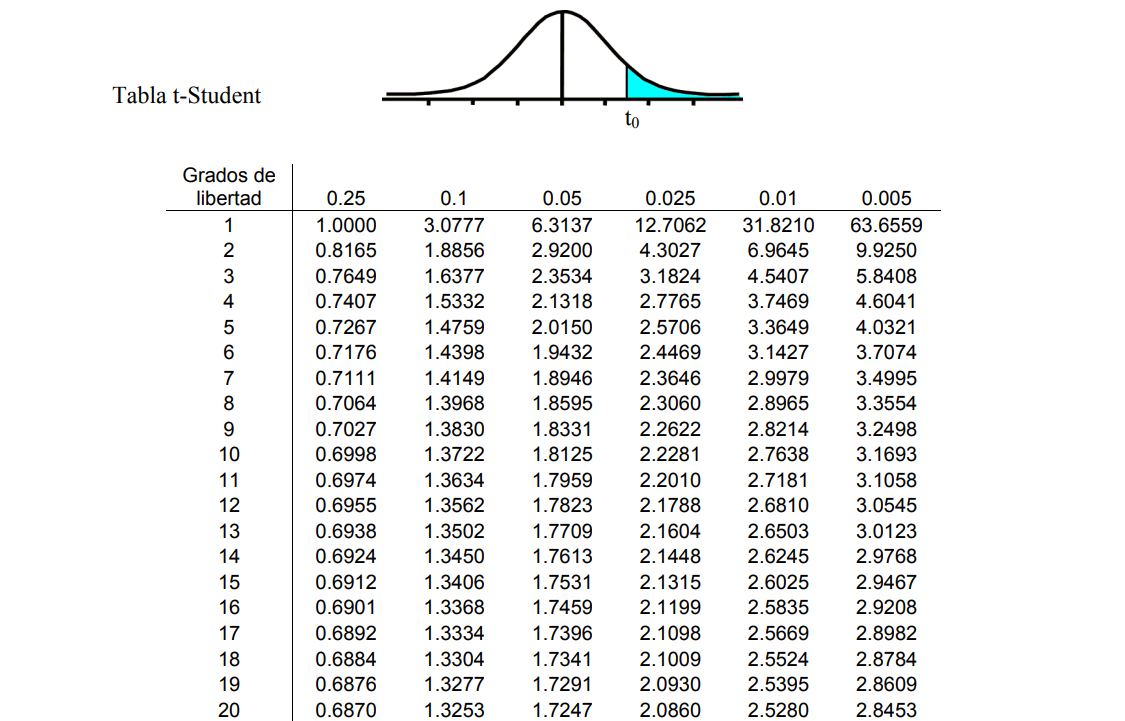
\includegraphics[scale=0.4]{T-Student.png}
\end{center}

\end{frame}
}

{
\setbeamercolor{background canvas}{bg=yellow!10}
\begin{frame}[fragile, plain]
\frametitle{\textsc{Inferencia Estadística}}
\setbeamercolor{item}{fg=blue}
\setbeamercolor{normal text}{fg=gray!40!black}
\usebeamercolor[fg]{normal text}
\hspace*{-5mm}
\vspace*{-5mm} 

$$Prob [-2.2622<\frac{\hat\alpha-\alpha}{se(\hat\alpha)}<2.2622]=0.95$$
$$Prob [-2.2622*se(\hat\alpha)-\hat\alpha<-\alpha<2.2622*se(\hat\alpha)-\hat\alpha]=0.95$$
$$Prob [\hat\alpha-2.2622*se(\hat\alpha)<\alpha<\hat\alpha+2.2622*se(\hat\alpha)]=0.95$$
$$Prob [55.85268-2.2622*14.49125<\alpha<55.85268+2.2622*14.49125]=0.95$$
$$Prob [23.0711823<\alpha< 88.6341681]=0.95$$

$$Prob [-2.2622<\frac{\hat\beta-\beta}{se(\hat\beta)}<2.2622]=0.95$$
$$Prob [0.2505531<\beta<  0.3733728]=0.95$$



\end{frame}
}

{
\setbeamercolor{background canvas}{bg=yellow!10}
\begin{frame}[fragile, plain]
\frametitle{\textsc{Test de Hipótesis}}
\setbeamercolor{item}{fg=blue}
\setbeamercolor{normal text}{fg=gray!40!black}
\usebeamercolor[fg]{normal text}
\hspace*{-5mm}
\vspace*{-5mm} 

\textbf{Modelo:}   $Y=\beta_1 + \beta_2 X + \mu$ \\

\textbf{Hipótesis Nula:}   $H_o: \beta_2 = \beta_2^0$ \\

\textbf{Hipótesis Alternativa:}   $H_1: \beta_2 \neq \beta_2^0$

\texttt{Esta secuencia requiere el testear hipótesis al 5\% y al 1\% de niveles de significancia. Para probar las hipótesis asumimos que la pendiente es igual a un valor $\beta_2^0$. Como vemos lo que requerimos es probar la hipótesis nula contra una alternativa que indica que el coeficiente es diferente de dicho valor}. \\
\vspace{0.1cm}

\hrule  

\vspace{0.1cm}

\textbf{Modelo:}   $p=\beta_1 + \beta_2 w + \mu$ \\

\textbf{Hipótesis Nula:}   $H_o: \beta_2 = 1$ \\

\textbf{Hipótesis Alternativa:}   $H_1: \beta_2 \neq 1$

\texttt{Se relaciona el crecimiento de los precios con el de los salarios. La hipótesis nula es que si los salarios crecen en 1\%, la inflación crece en ese mismo porcentaje (También podríamos probar la significancia estadística del coeficiente $\beta_2=0$)}

\end{frame}
}

{
\setbeamercolor{background canvas}{bg=yellow!10}
\begin{frame}[fragile, plain]
\frametitle{\textsc{Test de Hipótesis}}
\setbeamercolor{item}{fg=blue}
\setbeamercolor{normal text}{fg=gray!40!black}
\usebeamercolor[fg]{normal text}
\hspace*{-5mm}
\vspace*{-5mm} 

\texttt{La hipótesis nula asume que el coeficiente $\beta_2$ cuenta con una distribución con media 1 y desviación estandar de 0.1 (esto lo estamos asumiendo para este ejercicio). Para rechazar la hipótesis nula la probabilidad de obtener un estimador de 1 debe ser menor del 5\%. De acuerdo con ello, la regla de decisión conlleva a que rechacemos la hipótesis nula  si el estimador cae en el 2.5\% de la cola inferior o superior. Por lo regular el 2.5\% de las colas de una distribución normal se encuentran 1.96 desviaciones estándar de su media.}
\vspace{0.1cm}

\hrule  

\vspace{0.1cm}
\textbf{Rechazamos la hipótesis nula si el valor calculado se encuentra 1.96 desviaciones estandar ( o más) por encima o por debajo de la media hipotética}

\textbf{\underline{Regla de decisión al 5\% del nivel de significancia:}}

Si $\frac{(\beta_2 -\beta_2^0)}{sd}>1.96$  Si $\frac{(\beta_2 -\beta_2^0)}{sd}<-1.96$

\vspace{0.1cm}

Si $z>1.96$  Si  $z<-1.96$

\vspace{0.1cm}

\hrule  

\vspace{0.1cm}

\texttt{En el caso de 1\% el valor crítico es de 2.58}

\end{frame}
}


\end{document}


